\documentclass[sigconf,screen,9pt]{acmart}

% Flag to disable all editing macros and make the document ready for
%  submission.
\newif\ifEditMode

% Editing mode.
\EditModetrue
% % Submission mode.
% % The `submission' mode merges certain comments and edits, and removes some
% % other notes, TODOs and remarks. For more details, refer to the `reviewing
% % macros' in the `vusec.sty' file.
%\EditModefalse

\usepackage{paralist}
\usepackage{vusec}
\usepackage{frontmatter}
\usepackage{aliases}
\usepackage{listings}
\usepackage{minted}


\begin{document}


%% Thesis title.  Mitigations of hypervisor detection techniques in Windows using HyperDbg in its transparency mode
\newcommand{\thesistitle}{Mitigations of hypervisor detection techniques in Windows using HyperDbg}


%% Author information.
%% (Used in a couple of places, so it's better to define them in one place.)
\newcommand{\thauthor}{Mārcis Zariņš}
%%  Student number.
\newcommand{\thauthorid}{2781630}
\newcommand{\thauthoremail}{m.zarins@student.vu.nl}
\newcommand{\thauthoraff}{Vrije Universiteit Amsterdam}


%% Thesis type.
%% Valid values are `vubachelor', `csmaster', `pdcsmaster', `csecmaster', and `litstudy'.
%%
\thtype{vubachelor}

%% Course code.
\thcc{XB\_40001}

%% Thesis title.
\thtitle{\thesistitle}

%% Paper/thesis author.
\thauthname{\thauthor}
\thauthid{\thauthorid}

%% First supervisor.
\thsvfirst{Erik van der Kouwe}{Dr.}

%% Daily supervisor.
\thsvdaily{Mohammad Sina Karvandi}{MSc.}

%% Second daily supervisor.
%% \thsvdaily{Björn Ruytenberg}{MSc.}

%% Second reader.
\thrdrsecond{Mohammad Sina Karvandi}{MSc.}

\pagenumbering{gobble}
%% Attach customize front matter.
\addfrontmatter{}


\title{\thesistitle}

\author{\thauthor}
\affiliation{
  \institution{\thauthoraff}
  \city{Amsterdam}
  \country{NL}
}
\email{\thauthoremail}


\begin{abstract}
Dynamic analysis of malware is commonly performed in a virtualized environment, managed by a hypervisor. 
This keeps it isolated from hardware and the analysis can stay hidden and detached from the system. But the hypervisor is not completely hidden and malware using anti hypervisor 
detection methods can still detect the virtual environment and evade analysis and detection. 

In this thesis we look into the hypervisor detection methods malware use as well as design mitigations for them.  
We then integrate these mitigations into a transparency mode in HyperDbg, a debugging tool based on a hypervisor. With these mitigation features in HyperDbg, 
we evaluate the effectiveness of them by deploying them against multiple hypervisor detection tools that compile numerous detection methods used by malware and execute them, 
attempting to detect a hypervisor. We show that, while perfect transparency is not achieved, there is a noticeable improvement in hypervisor transparency.



%%% Local Variables:
%%% mode: latex
%%% TeX-master: "../thesis"
%%% End:

\end{abstract}

\maketitle

\pagenumbering{arabic}

\section{Introduction}\label{s:intro}

\stress{Think before you write, be careful how you write, and take feedbacks
seriously}~\cite{Heiser-WebArticle2022}.


This section includes some motivations behind the work, explicitly or implicitly
highlights the research question, provides a high-level explanation of the
solution, and describes the contributions.

\textcolor{lightgray}{\lipsum[1]}

\parai{Makefile.}
%
It is typical to build a PDF from the \LaTeX{} sources using \texttt{make}, but
resist the temptation to fill the \texttt{Makefile} with complex and unnecessary
rules or recipes.
%
You only need one line, where you invoke \texttt{latexmk}.
%
This template should also come bundled with a \texttt{Makefile}, which should
suffice in virtually all scenarios.

\textcolor{lightgray}{\lipsum[3-4]}

\begin{figure}[tbh]
    %% The macro `\onecolgrid' is defined in `vusec.sty'
    %% NOTE: The suffix "./figs/" is implicitly included for this relative path.
    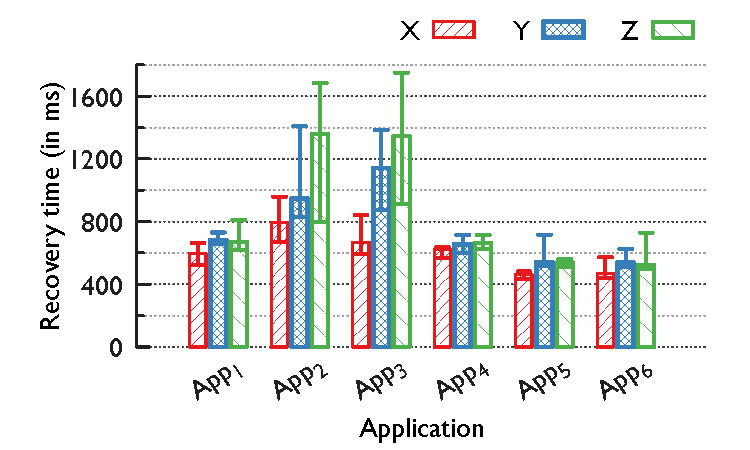
\includegraphics[width=\onecolgrid]{cache-by-app}
    %% Labels should immediately follow caption, to keep latex quiet.
    \figcap{Simple one-column figure. Please include a brief explanation or
    takeaway.}\label{fig:1col}
\end{figure}

\parai{Figures.}
%
Do not include figures that you do not refer to or discuss in the text.
%
Generate high-quality figures (Fig.~\ref{fig:1col})---think PDF or EPS.
%
With the number of tools and libraries that are available today for generating
beautiful plots, there is no excuse for producing ugly plots.
%
Figure caption must go at the bottom of a figure (Fig.~\ref{fig:3col}), and it
is also a good place to highlight the key takeaway of that figure.
%
Avoid using the position parameters `p' and `!', unless you are absolutely sure
that is exactly what you want.

\begin{figure*}[th]
    %% The macro `\threecolgrid' is defined in `vusec.sty'
    \begin{subfigure}[t]{\threecolgrid}
        %% NOTE: The suffix "./figs/" is implicitly included for these relative paths.
        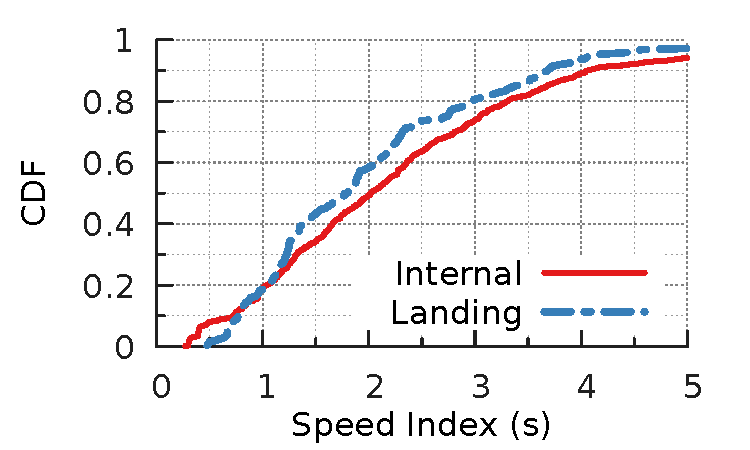
\includegraphics[width=\linewidth]{three-col/speed_index}
        \sfigcap{}\label{fig:3col-a}
    \end{subfigure}
    \begin{subfigure}[t]{\threecolgrid}
        %% NOTE: You do not have to mention the extension.
        %% (The example figures are in PDF format.)
        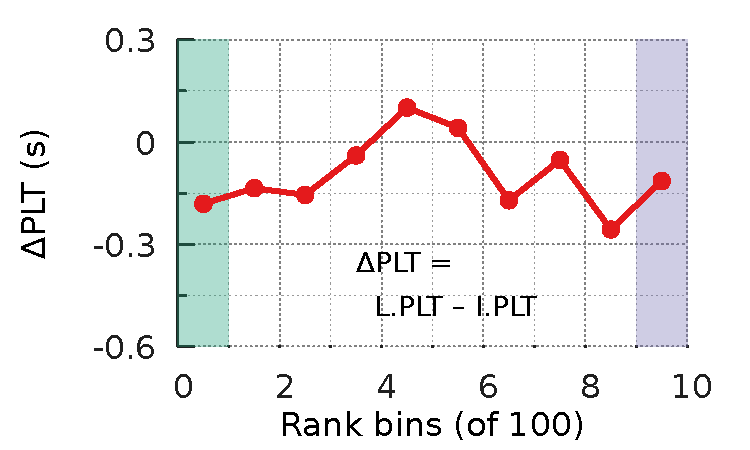
\includegraphics[width=\linewidth]{three-col/plt_ranks_diff}
        \sfigcap{}\label{fig:3col-b}
    \end{subfigure}
    \begin{subfigure}[t]{\threecolgrid}
        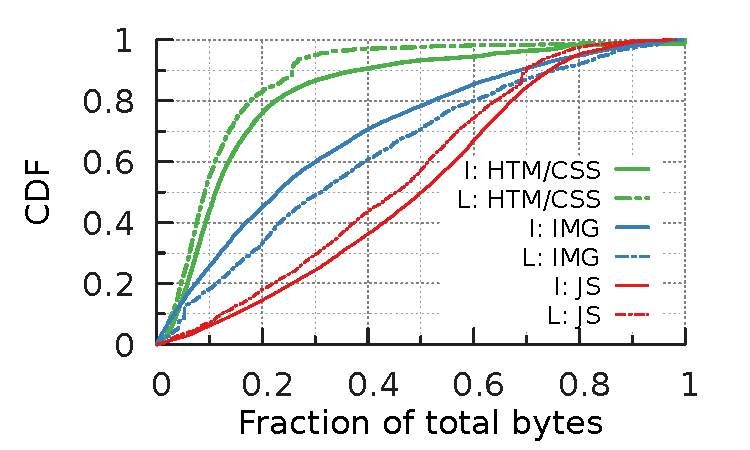
\includegraphics[width=\linewidth]{three-col/mimes}
        \sfigcap{}\label{fig:3col-c}
    \end{subfigure}
    %% Labels should immediately follow caption, to keep latex quiet.
    \figcap{Generate clear and beautiful figures (in PDF) that can be rendered side by side while still being easy to read and interpret. Choose colors wisely from the colorbrewer2.org website.}\label{fig:3col}
\end{figure*}

\textcolor{lightgray}{\lipsum[6-7]}

\begin{table}[tb]
    \centering
    \tabcap{A simple table describing the characteristics of a data set or the
    results of an experiment.}\label{tab:sample}
    \taburulecolor{black!45}
    \begin{tabu}{c|c|r|r|r|r}
        \toprule
        \multirow{2}{*}{\thead{Char.}} &
            \multirow{2}{*}{\thead{\#samples}} &
            \thead{Count} &
            \multicolumn{3}{c}{\thead{Perf. Score}}\\
        &
            &
            \thead{of items} &
            \thead{X} & \thead{Y} & \thead{Z} \\
        \midrule
        \stress{P}
            & 214 & 56 & 9 & 23 & 24 \\
        \stress{Q}
            & 117 & 27 & 7 & 10 & 10 \\
        \stress{R}
            & 222 & 11 & 6 & 4 & 1 \\
        \stress{S}
            & 187 &  9 & 1 & 6 & 2 \\
        \stress{T}
            & 180 & 16 & 7 & 5 & 4 \\
        \bottomrule
    \end{tabu}

\end{table}

\parai{Tables.}
%
The caption must go at the top of the table (Tab.~\ref{tab:sample}).
%
Do not use \texttt{\textbackslash{}hrule}.
%
Use \texttt{\textbackslash{}toprule} above the heading,
\texttt{\textbackslash{}midrule} below the heading, and
\texttt{\textbackslash{}bottomrule} below the last row.
%
You could also use \texttt{\textbackslash{}hrule} as a row separator.
%
Right align numerical values, and use math-mode for (large) numerical values to
force \LaTeX{} to use monospaced fonts and ensure right-alignment functions as
expected.

\textcolor{lightgray}{\lipsum[12-14]}

We summarize our contributions as follows.

\case{}
%
\textcolor{lightgray}{\lipsum[10][2-4]}

\case{}
% 
\textcolor{lightgray}{\lipsum[11][4-8]}

\case{}
% 
\textcolor{lightgray}{\lipsum[12][2-6]}

\case{}
% 
\textcolor{lightgray}{\lipsum[16][4-8]}

Depending on your degree program and/or supervisor, you may need to furnish the
“Artifact Appendix” (\S\ref{s:appendix}).


%%% Local Variables:
%%% mode: latex
%%% TeX-master: "../thesis"
%%% End:

\section{Background}\label{s:background}

This section provides the necessary context to help the reader understand the
remainder of the thesis.


Theory behind virtualization(most are lvl2, HyperDbg is lvl1), that it can be detected. mention of the use in malware analysis


%%% Local Variables:
%%% mode: latex
%%% TeX-master: "../thesis"
%%% End:

%%\section{Threat Model}\label{s:threat-model}

Use this section to address key questions: (a) What does this thesis or paper
assume about the attackers’ goals and objectives? (b) What do you assume about
the systems and their environment, etc.

\textcolor{lightgray}{\lipsum[7-11]}


%%% Local Variables:
%%% mode: latex
%%% TeX-master: "../thesis"
%%% End:

\section{Overview}\label{s:overview}

\subsection{Detecting a hypervisor}\label{HV_detection}

Although hypervisors by design are not easily detectable, there still exist many ways to detect the presence of them from the user-space level. 
This thesis could not cover all of the possible detection ways, but it does touch on the most commonly used methods.

%% Might look better to add a subsection for each of these parai sections(CPUID and RDTSC combined as x86 ASM instructions)
\parai{CPUID}
One of the most commonly used detection methods involves querying the CPUID instruction, defined in the x86 architecture. 
This instruction returns information about the CPU and has multiple fields in the return data from which hypervisor identifiable information can be obtained. 
A more exhaustive explanation of this instruction can be found in the Intel\textsuperscript{\tiny\textregistered} 64 and IA-32 Architectures Software Developer's Manual~\cite[Volume~2A]{Intel-SDM2025}. 

Under a hypervisor, this instruction will always cause an unconditional VM-exit, and the hypervisor must have a handler present to correctly handle the instruction, 
which in most cases can be a passthrough to the logical CPU. Calling this instruction and reading specific bits of the return data is the easiest 
and most common way a process can detect the hypervisor, but this relies on the hypervisor itself writing this identifiable data before returning from the VMX root mode. 
A transparent hypervisor can be set up to pass through the instruction to the logical CPU for every query, and the guest system could never detect this hypervisor from only the CPUID instruction.

\parai{RDTSC}
Another x86 instruction that causes an unconditional VM-exit in a virtualized environment is the RDTSC instruction. This instruction reads and returns the value of the time stamp counter, 
a register that counts the CPU cycles since its reset. Its use in hypervisor detection is also common, as it allows the detection of timing anomalies introduced by the aforementioned VM-exits 
and other transitions between non-root and root modes~\cite{hyperdbg-transparency}. This instruction can be called twice, before and after another instruction that causes a VM-exit, like CPUID, to obtain an aproximate CPU
cycle count this instruction took to execute. Subtracting values returned by the RDTSC instructions would show detectable overhead as the mode transitions, as well as the hypervisor itself, 
will execute more instructions and spend more CPU cycles than executing the same code in a bare metal system. 
As seen in Figure~\ref{fig:rdtsc_overhead}, the CPU cycle count required to execute the CPUID instruction is much larger when run in a VMWare virtualized environment than on bare metal. 
\begin{figure}[tbp]
    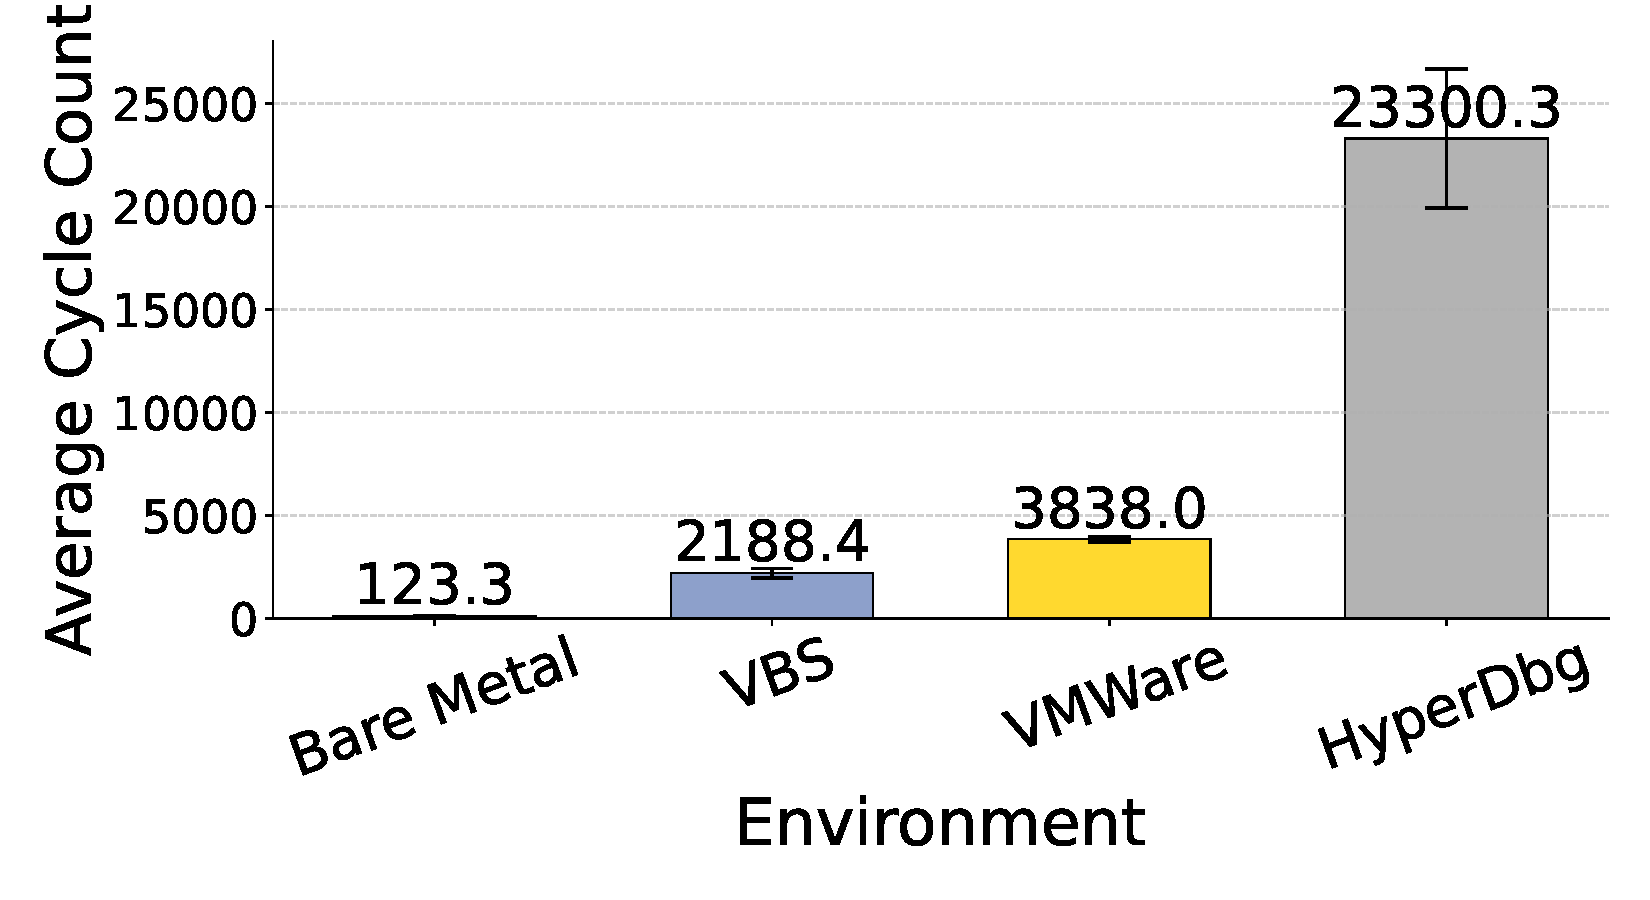
\includegraphics[width=\onecolgrid]{RDTSC_execution} %RDTSC_execution
    \figcap{Average cycle count of executing CPUID instruction in 4 different environments. VBS was tested on the same bare metal system and HyperDbg was run on top of a VMware system}\label{fig:rdtsc_overhead}
\end{figure}

It is also visible that HyperDbg's implementation of the CPUID instruction handler or the general VM-exit handler is less efficient than VMWare's implementation, as the cycle count overhead is over 5 times larger. 
This VM detection method is reliable, as the overhead measurements are done in cycle count not time offset, and it is hard to defeat from the hypervisor, as many genuine processes rely on the RDTSC 
instruction. The detection is also done as a pattern not a singular query, making detecting the attempt of hypervisor detection unreliable and hard to implement~\cite{hypervisor-detection-timing-attacks}. 
The viability of this detection method, however, is no longer that high. In recent Windows operating system releases, Microsoft has introduced Virtualization Based Security (VBS) feature~\cite{windows-vbs} 
that runs the operating system on top of a light-weight hypervisor. This feature is enabled by default on modern Windows systems and introduces almost the same cycle count overhead (see Figure~\ref{fig:rdtsc_overhead}). 
Malware that wants to target as many systems as it can or bypass this security feature would have to sacrifice using the aforementioned detection method as it would blacklist and not deploy on not just the virtualized systems used for its analysis, 
but most bare metal systems as well. It should be noted that the overhead is smaller than that of the other hypervisors tested, but the difference is small, and differentiating them would be less reliable from the detection point of view.
The popularity of containerized environments, especially for servers, also adds to the low reliability of this detection method if the goal is to deploy on as many systems as possible.

\parai{System calls}
When focusing on a specific guest operating system, detecting hypervisors can be done by using system calls provided by the OS. 
On Windows, there are numerous ways how system calls could be used to assist in detecting them. This thesis focused on the Windows system calls seen in Table~\ref{tab:syscalls}. 

These system calls were chosen based on the data they return, by analysing the return data when called on a VM and looking if it contains any information that could be used for detecting this VM. Some system calls were also chosen
to be mitigated based on their common use in hypervisor detection tools.
For the specific system call numbers J00ru's Windows x64 system call table~\cite{j00ruSyscalls} was used. These call numbers are based on Windows 11 version 24H2. All of them can be invoked from a user-space process, and can reveal the presence of a hypervisor in some way. 
Many of the calls focus on file and registry key access as commercial hypervisor vendors write identifiable data to the guest system. 
There are many mitigations to these attempts of detection~\cite{yang2024makingsyscallprivilegeright, 11027539}, but the design developed as part of this thesis focuses on intercepting the system calls at the OS kernel level 
and modifying the data the calling process receives if it contains hypervisor identifying data.

Although these mitigations themselves try to stay hidden from the caller processes and the hypervisor might be transparent from the detection attempts, intercepting these calls comes with some trade-offs that allow user processes to detect that
some intervention was performed; this will be discussed in more detail in Section~\ref{syscall_interception}.
For these mitigations, some system calls only require changing the return value, while others need intercepting pointers to user-allocated buffers from the system call arguments and modifying the data inside these memory addresses.
The main issue with the use of system calls in hypervisor detection is that they are bound to a single operating system, and in the case of Windows possibly to a single version, as Microsoft tends to change the system call numbers over versions.
This version limitation, however, can be bypassed by using Windows API function calls for the wrapper functions of the system calls, but this approach is considerably more easier to mitigate and can even be done in user space, without a need for hypervisor intervention.
However, the mitigations themselves could also be bypassed if they were implemented in user space, as will be shown in Section~\ref{scyllahide-comparison}.

\begin{table}[tb]
    \centering
    \tabcap{Some Windows systemcalls with a possible use in hypervisor detection}\label{tab:syscalls}
    \taburulecolor{black!45}
    \begin{tabu}{l|c|c|c|c}
        \toprule
        \multirow{2}{*}{\thead{Name}} &
            \thead{System call} &
            \thead{Implemented} \\
        &
            \thead{number in 24H2} &
            \thead{in HyperDbg}\\
        \midrule
        NtQuerySystemInformation
            & 0x0036 & \checkmark \\
        NtSystemDebugControl
            & 0x01D0 & \checkmark\\
        NtQueryAttributesFile
            & 0x003D & \checkmark \\
        NtQueryObject
            & 0x0010 &\\
        NtOpenDirectoryObject
            & 0x0058 &\\
        NtQueryDirectoryObject
            & 0x014E & \checkmark\\
        NtQueryInformationProcess
            & 0x0019 & \checkmark \\
        NtQueryInformationThread
            & 0x0025 &\\
        NtOpenFile
            & 0x0033 & \checkmark\\
        NtOpenKey
            & 0x0012 & \checkmark \\
        NtQueryValueKey
            & 0x0017 & \checkmark \\
        NtEnumerateKey
            & 0x0032 & \checkmark \\
        NtUserFindWindowEx
        & 0x1067 &\\
        NtUserBuildHwndList
        & 0x101A &\\
        \bottomrule
    \end{tabu}

\end{table}

\parai{Model specific registers.}
Model specific registers (MSR) are special registers defined on the CPU that can be accessed only via special RDMSR and WRMSR instructions~\cite[Volume~4]{Intel-SDM2025}.
These MSRs contain different and more detailed data than the information that can be obtained using the CPUID instruction, as well as specific control register fields. 
Importantly for hypervisor detection, the behavior of accessing specific MSR addresses or ranges is different when the system is virtualized, 
as both the read and write instructions cause unconditional VM-exits and are handled by the hypervisor. Due to these instructions also being limited to privilege ring 0, 
MSR access patterns are not as common as detection vectors, but if they are used, a positive test result guarantees a definitive detection of a hypervisor.

\parai{Other detection methods.}
This thesis only focuses on a small number of hypervisor detection methods and their mitigations. There are many more ways to detect the presence of a virtual environment and as many ways to mitigate this.
Some other detection vectors might include checking I/O and other hardware device IDs and properties, reading the names of the system or the user account, checking system firmware data or executing hypervisor specific detection tests.
Mitigating all possible detection methods is almost impossible, but at the same time, implementing and executing all these virtualization detection methods is inefficient in both time and space and can cause higher rates of false positives.


\subsection{Design approach}\label{design_approach}
Due to the complexity of the mitigations for some of these detection methods and the scope of this thesis, only 3 general approaches to detection were handled: CPUID queries, MSR access patterns, and Windows system calls. 
The hypervisor detection mitigation features were implemented into HyperDbg's transparency mode. 

When HyperDbg is deployed on a system, the transparency features, and thus the ability to hide any hypervisors from detection, is disabled. To enable the transparent mitigations, 
once HyperDbg is connected in kernel debug mode, \textbf{\texttt{!hide}} command needs to be entered. This enables all hypervisor detection mitigations that were implemented as part of this thesis and, 
as it will be shown in the Evaluation section, improves the stealthiness of the hypervisors present. An overview of the deployment of the transparent mitigations with HyperDbg can be seen in Figure~\ref{fig:hyperdbg_overview}.

\begin{figure*}[t]
    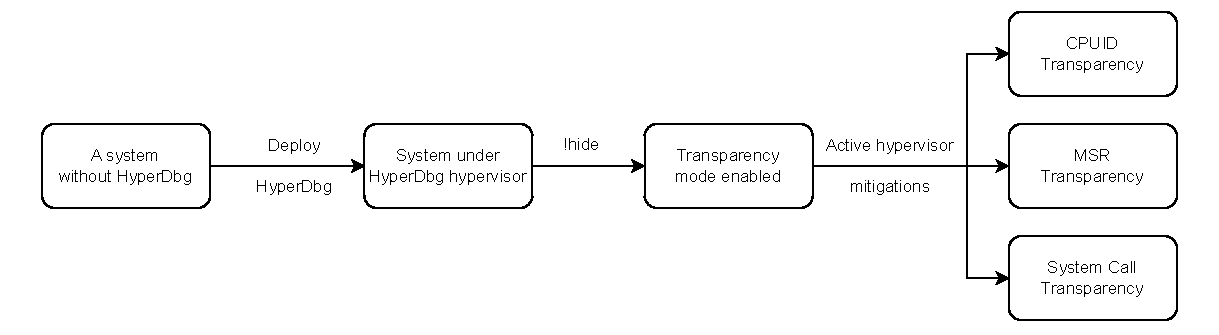
\includegraphics[width=\textwidth]{HyperDbg_diagram} %RDTSC_execution
    \figcap{Diagram of deploying the hypervisor transparency features implemented in HyperDbg}\label{fig:hyperdbg_overview}
\end{figure*}


%%% Local Variables:
%%% mode: latex
%%% TeX-master: "../thesis"
%%% End:

\section{Transparency Feature Design}\label{s:design}

\subsection{General Overview}
This chapter describes the design choices of the mitigation methods in HyperDbg that were made during this project. The design was made for the development of HyperDbg, and focused on its transparency mode. 
As already mentioned before in section~\ref{design_approach}, due to feasibility and time constraints, only a handful of the mitigations were developed. 
These include return value adjustment of the CPUID instruction, behaviour modification of certain MSR accesses and the hooking and interception of Windows kernel system calls. 
The implementation was done based on HyperDbg's 0.13.0 version, on a GitHub fork of the project\footnote{The repository of the forked HyperDbg project, where the implementation was done available at: \url{https://github.com/CokeTree3/HyperDbgThesis}}.

The design was made to be deployable on any system, but the implementation and testing, and thus a guarantee of reliability, was performed on a Windows 10(22H2) bare metal system running on an Intel CPU that supports VT-x hardware virtualization. 
The deployment and further evaluation was performed in a nested virtualization environment, where HyperDbg hypervisor driver was deployed over a VMWare Workstation 16 virtual machine. 
This VM was running Windows 10 version 22H2 as the operating system. For reliability of the design, all testing and evaluation was also performed on an identical virtual machine, but one that is running Windows 11 version 24H2.

\subsection{Feature Design}
\subsubsection{CPUID}
As described by Microsoft\footnote{CPUID instruction description in terms of hypervisor discovery. Microsoft \url{https://learn.microsoft.com/en-us/virtualization/hyper-v-on-windows/tlfs/feature-discovery}}, 
there are 2 ways the CPUID instruction can be used to check hypervisor presence, reading the “hypervisor present” bit that is at 31 bit offset of the leaf 0x1, that is, the instruction queried with the EAX register set to this value.
\begin{minted}[linenos,frame=single]{nasm}
    MOV EAX, 0x1
    CPUID
\end{minted}
Or by querying the 0x40000000 leaf for the vendor identifier and max defined leaf range above the 0x40000000 leaf. 
\begin{minted}[linenos,frame=single]{nasm}
    MOV EAX, 0x40000000
    CPUID
\end{minted}
Without mitigations, after calling CPUID, registers EBX, ECX and EDX will contain the hypervisor vendor string, if it is set as such by the hypervisor.
Both of these methods can be mitigated by intercepting the unconditional VM-exit caused by the CPUID instruction, and changing the return values in RAX, RBX, RCX and RDX registers. 
By just unsetting the 'hypervisor present bit' in RAX, if the query request in RAX is 0x1, leaving RAX at value 0x4000000, to indicate no higher leaves are defined, and not setting the vendor identifier in the other registers.

\subsubsection{Model Specific Registers}
Similarly, MSR accesses can also be mitigated. Intel defines MSR's in the range 40000000H - 4000FFFFH as reserved~\cite[Volume 4]{Intel-SDM2025} and so they are guaranteed to not be used by hardware. 
Due to this, Microsoft defines them as “Synthetic model specific registers”~\cite{microsoft_hv_interface_reqs}, and consumer hypervisors that conform to the Hyper-V \stress{Hv\#1} interface must define some MSR's in this range. 
In a bare metal system any access to an undefined MSR causes a general protection error (\stress{\#GP}). In the design, this behaviour was emulated, 
so whenever the transparency mode is enabled within HyperDbg, any reads or writes to/from this range, will cause a \stress{\#GP} error to be injected to the guest.

\subsubsection{Windows system call interception}\label{syscall_interception}
For the interception and modification of Windows system calls, the approach chosen was to insert an EPT page hook (A feature already implemented in HyperDbg before this paper) 
at the entry point of Windows system call handler function KiSystemCall64, which is the function that performs the privilege level swap between user-mode and kernel-mode. 
Access to the location of this function is obtained from the IA32\_LSTAR MSR. 
This allows HyperDbg to intercept all calls to this function by causing an unconditional VM-exit and filter the system calls based on their system call number. 
The call number is stored in the RAX register as set up by the user-mode system call wrapper functions in the \stress{NTDLL} library~\cite{ntdll-lib}. The general style of these 
wrapper functions are as shown in Listing~\ref{lst:syscall-wrapper}, but with the system call number changed to the appropriate one.
This disassembly also shows that the wrappers move the second argument of the system call, as defined by the used x64 fastcall calling convention, 
to R10 from the standard RCX register. This was a detail that was considered during the development.

At the point when the EPT hook is triggered, the system has just transferred the context to kernel-mode and no execution relating to the requested system call has been done. 
To get to a point in the execution path where data has been written to any memory buffers or the return values have already been set, 
requires returning control back to the guest system and intercepting the execution path once more, before the control is passed back to the calling user-mode process or API function. 
The approach chosen was to set the trap flag in the guest-mode RFLAGS register for the specific thread, which during the interception point is stored on R11. 
Once the execution returns to user-mode via the SYSRET instruction, and the user-mode RFLAGS are restored, the first instruction will immediately trigger a software interrupt, due to the TRAP flag
being set. HyperDbg catches this interrupt and gives an opportunity to access and modify the return value the user-mode process will be receiving from the system call. 
As many system calls also provide data, more than just a return value, at this point HyperDbg also can read and modify any memory buffers that were 
passed as arguments when the system call was invoked. This callback approach to system call interception allows HyperDbg to filter and only intercept 
the offending system calls, Table~\ref{tab:syscalls} and greatly improves performance over intercepting and causing VMX mode changes multiple times on every system call made.

\subsubsection{Modification of system call behaviour}
Once the system calls can be intercepted, the chosen non-transparent calls are filtered and an entry handler for each one can be created. 
These functions execute at the entry point of the system call execution in the kernel, as triggered by the EPT page hook. 
These handlers range from simply setting the trap flag for all calls to the specific system call, to reading user-mode buffers written by the caller process, 
filtering the kernel access calls even further. The handler might also corrupt some register values, to trigger an error code to be generated by the kernel 
instead of executing the requested data query. As an example, the Windows system call NtQueryAttributesFile\footnote{NtQueryAttributesFile system call. Microsoft. \url{https://learn.microsoft.com/en-us/windows/win32/devnotes/ntqueryattributesfile}}, 
which retrieves basic information on a specific file or a directory, requires 2 arguments: an input structure and a buffer to write the queried information to.
A process attempting to detect a hypervisor might execute this system call on a number of common files that commercial hypervisor vendors might add to a guest system, 
as well as driver files present in the system. The approach taken for mitigating this is to report errors when a query for a known hypervisor specific file is being accessed. 
To achieve this, the system call entry handler has to read the input structure from the user-mode virtual pointer, check if the call is a query for these \stress{"bad"} files, 
and only then deploy the mitigation. Which in this case is to set the trap flag and resume the kernel execution, 
as the actual mitigation has to happen after the kernel returns to user-mode.

Once the kernel executes the SYSRET instruction, and returns to user-mode, the inserted trap flag causes another VM-exit and based on the system call number stored in a list, 
another handler can be called for this callback. At this point in the execution path of system calls, the return value has already been set on RAX and the user-mode buffers 
have been written to, if required, by the kernel. This allows the transparent mitigation handlers to read these buffers and modify any data in them 
that could reveal hypervisor presence, like removing active processes and loaded drivers from their respective lists, 
or spoofing the vendor identification in Windows registry key or firmware data.
The mitigations take place in VMX root mode, operating at level -1 and since these pointers given in the arguments are from the calling processes (level 3) virtual address space, 
accessing them directly is not possible, so a translation layer needs to be added. The method chosen was to read and copy the data from the translated physical address to a spare memory buffer, 
either on the stack or to an allocated non-paged memory on the heap. From there, modifications of the data in these buffers could be performed, as required based on the system call, 
and then written back to the user-mode buffer physical address.
The return values are aalso spoofed at this point, if needed, by updating RAX register value. In most cases is is to set the value as an error code instead of the success code of 0x0. 

NtQuerySystemInformation is a system call that can retrieve many types of information on the system, the query is defined by an argument, 
a class value from the \stress{SYSTEM\_INFORMATION\_CLASS} enumeration defined in the NT API~\cite{ntdll-lib}. 
While not all of the class data could contain hypervisor revealing data, some of them do. The designed system call interception system mitigates many 
but not all of the query classes. Seen in Table, are a list of the \stress{SYSTEM\_INFORMATION\_CLASS} classes that could be used for hypervisor detection.

\begin{table}[tb]
    \centering
    \tabcap{Some SYSTEM\_INFORMATION\_CLASS classes with a possible use in hypervisor detection}\label{tab:QSI-classes}
    \taburulecolor{black!45}
    \begin{tabu}{l|c|c}
        \toprule
        \multirow{2}{*}{\thead{Name}} &
            \thead{Class} &
            \thead{Implemented} \\
        &
            \thead{number} &
            \thead{in HyperDbg}\\
        \midrule
        SystemProcessInformation
            & 0x05 & \checkmark \\
        SystemModuleInformation
            & 0x0B & \checkmark \\
        SystemKernelDebuggerInformation
            & 0x23 & \checkmark \\
        SystemFirmwareTableInformation
            & 0x4C & \\
        SystemHypervisorInformation
            & 0x5B&\\
        SystemHypervisorDetailInformation
            & 0x9F &\\
        SystemProcessIdInformation
            & 0x58 &\\
        SystemCodeIntegrityInformation
            & 0x67 & \checkmark \\
        SystemHandleInformation
            & 0x10 &\\
        \bottomrule
    \end{tabu}

\end{table}

The values and the returned structures were obtained from the NT API documentation provided by the \stress{System Informer} project\footnote{Native API online documentation, based on the System Informer. \url{https://ntdoc.m417z.com/}}.

Multiple hypervisor detection methods commonly used, rely on querying for the system firmware and vendor data. On Windows many of these queries are carried out with system calls, 
allowing HyperDbg to intercept them. To appear genuine, when the transparency mode is enabled, a random genuine vendor is chosen from a preset list of numerous genuine computer system and component vendors. 
Any queries for data through system calls, that contain hypervisor vendor data, from any process will always report back the same spoofed vendor data, bypassing any hypervisor checks done by the user process.

In the context of Windows, one commonly used approach for obtaining system information is by using the Windows Management Instrumentation(WMI)\footnote{Windows Management Instrumentation documentation. Microsoft. \url{https://learn.microsoft.com/en-us/windows/win32/wmisdk/wmi-start-page}}.
This API provides the user an interface through which to query and modify many aspects of the operating system. 
Importantly, it can be used in parallel to direct system calls to obtain system information which might reveal the hypervisor~\cite{graeber2015abusing}.
For this paper, WMI related detection methods did not have mitigations developed as the layout of the WMI structure is relatively spread out and 
does not interact with the kernel through an easily detectable system call, frequently not going through the kernel at all~\cite{wmi-structure}.

\subsection{Final design}
The designed system of hypervisor transparency is capable of intercepting 3 common detection vectors - CPUID instruction queries, accesses of certain MSR regions and Windows system calls - 
suppressing the ability for any user process or malware to successfully detect that they are running in a virtualized system and changing their execution paths. 

The design allows for a modular implementation, where each of the different mitigation handlers are independent to the other ones, 
while also being dynamic and allowing the transparency to be toggled on or off at runtime, not requiring a system restart for the guest.




%%% Local Variables:
%%% mode: latex
%%% TeX-master: "../thesis"
%%% End:

\section{Evaluation}\label{s:evaluation}

After the detection mitigation features were implemented in HyperDbg, the effectiveness of them was tested. The evaluation of the chosen design was tested in three 
different approaches. The effectiveness of the transparency was tested against publicly available, maintained tools that compile the numerous ways hypervisors 
and debuggers can be detected into one program and executes them all one by one, as well as comparing the interception approach of Windows system calls to 
ScyllaHide~\cite{scyllahide}, an anti-anti-debugging library that applies 
a similar style of transparency to debugger detection.

The evaluation also included overhead analysis, measuring the added time overhead introduced by the transparent mitigations.

For the effectiveness evaluation, code snippets were created and implemented into small console programs that executed a specific hypervisor detection technique 
and reported the result. These were used for both overhead analysis and for the comparison with ScyllaHide, which is also designed to spoof debugger presence.

The evaluation was done on a bare metal system with an Intel CPU which supports VT-x, as well as in a nested virtualization environment running on the same bare metal system, 
where the HyperDbg hypervisor driver was deployed over a VMWare Workstation 16 virtual machine. This VM as well as the host system were running Windows 10 version 22H2 as the operating system. 
For reliability of the design, the testing was also performed on a virtual machine running Windows 11 version 24H2, 
but this was done only for reliability testing and no further evaluation measurements were taken from this system configuration. 

\subsection{Overhead Analysis}
To evaluate the performance impact of the hypervisor mitigations implemented in HyperDbg, the time overhead was measured and analyzed. 
The measurements were taken from a C++ user-space program that measured the time difference before and after executing a function that executed the evaluated hypervisor detection method. 
Each detection method was tested 20 times, and to avoid any possible caching within the process, after each measurement the program was restarted. 
These tests covered CPUID instruction querying as well as multiple system call executions. Due to the testing taking place in user-space, 
MSR reads and writes could not be tested for their overhead due to MSR access being limited to privilege level 0~\cite[Volume 2B]{Intel-SDM2025}, and so could not be executed from user-space privilege level.
The implementation of the mitigations involving MSR access is in a similar style to the CPUID related mitigations, so the overhead is believed to be comparable to CPUID measurements.
The time data was collected with the C++ \stress{chrono} library, 
using the \stress{high\_resolution\_clock} class\footnote{C++ chono library, high\_resolution\_clock class. \url{http://www.en.cppreference.com/w/cpp/chrono/high_resolution_clock.html}}.
All of the measurements were taken from 4 environments: a bare metal system, a bare VMWare virtual machine, and the same 
VMWare environment with the HyperDbg hypervisor deployed over it, both with and without the transparency mode enabled.

As it can be seen in Figure~\ref{fig:cpuid_exec_time} executing the CPUID instruction with the mitigations enabled, as expected, did not cause noticeable time overhead. 
This is due to the fact that mitigations for this detection method do not add any additional code to the hypervisor and other than changing the returned value, the execution path does not change.
The overhead introduced by virtualization in the execution time is discussed in section~\ref{HV_detection}.
\begin{figure}[tbh]
    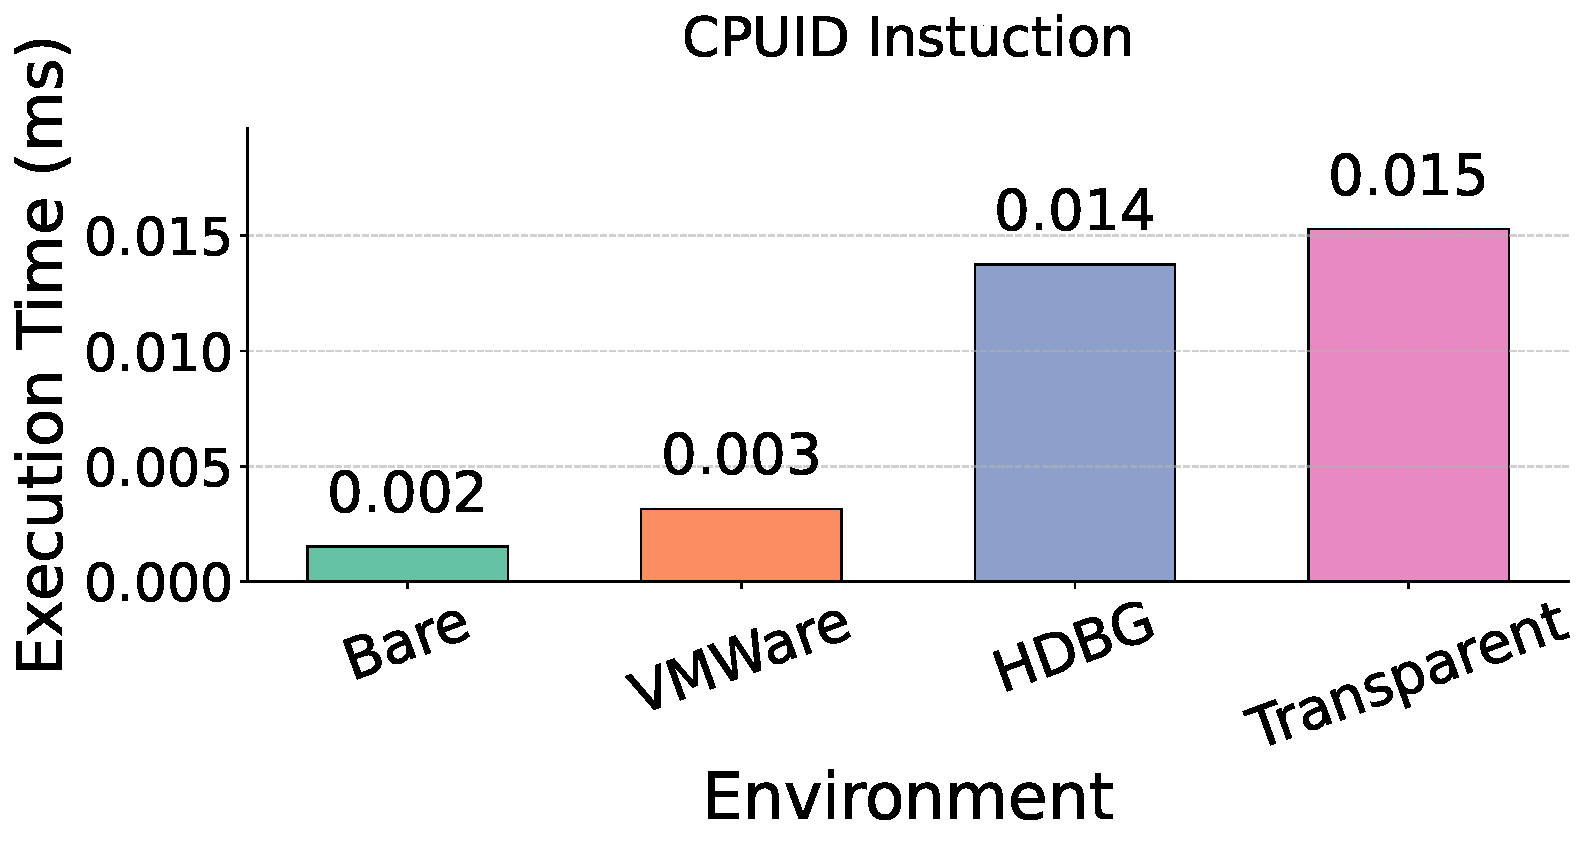
\includegraphics[width=\onecolgrid]{CPUID execution} %RDTSC_execution
    \figcap{Execution time of the CPUID instruction in different environments. HyperDbg is shortened to \stress{HDBG}, and the data for the detection mitigation transparency mode is labeled as \stress{Transparent}.}\label{fig:cpuid_exec_time}
\end{figure}

\begin{figure*}[th]
    \begin{subfigure}[t]{\threecolgrid}
        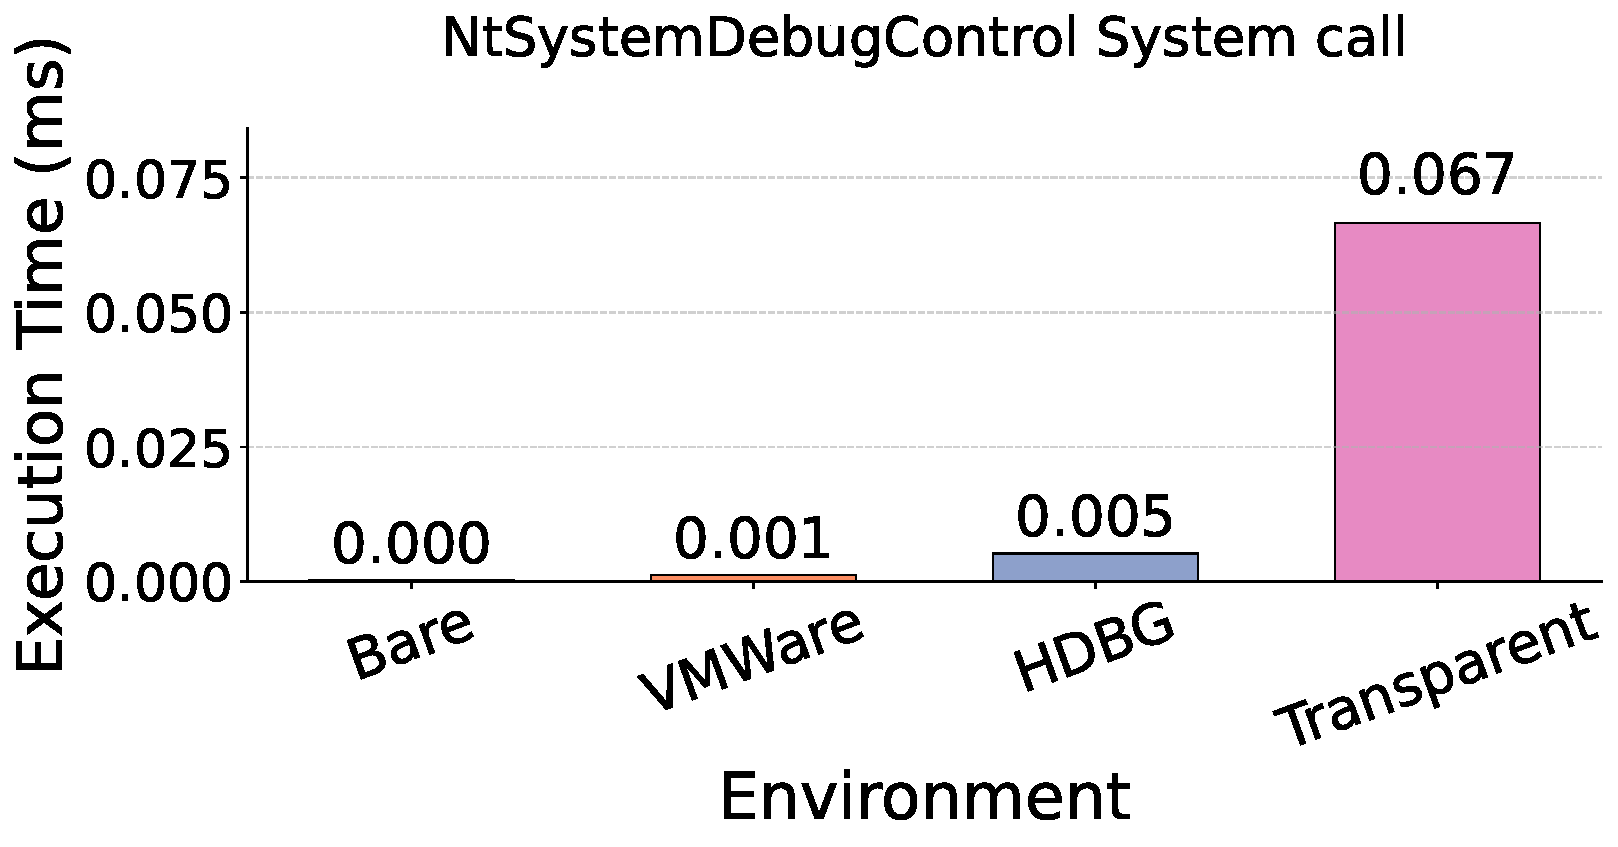
\includegraphics[width=\linewidth]{SDC execution}
        \sfigcap{}\label{fig:exec-time-a}
    \end{subfigure}
    \begin{subfigure}[t]{\threecolgrid}
        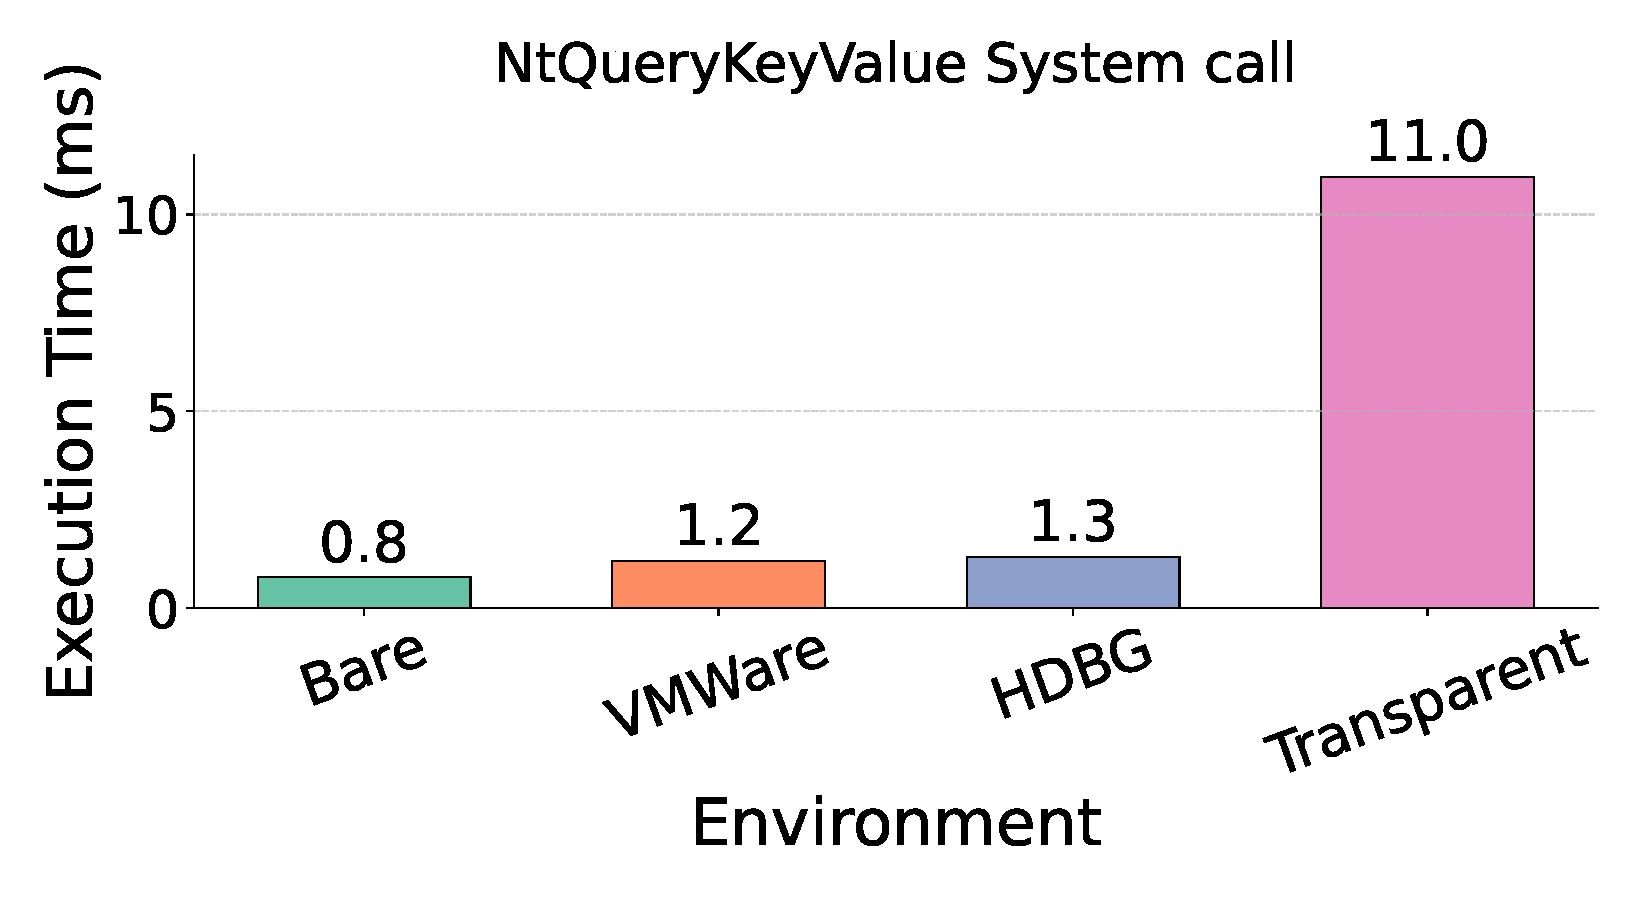
\includegraphics[width=\linewidth]{QKV execution}
        \sfigcap{}\label{fig:exec-time-b}
    \end{subfigure}
    \begin{subfigure}[t]{\threecolgrid}
        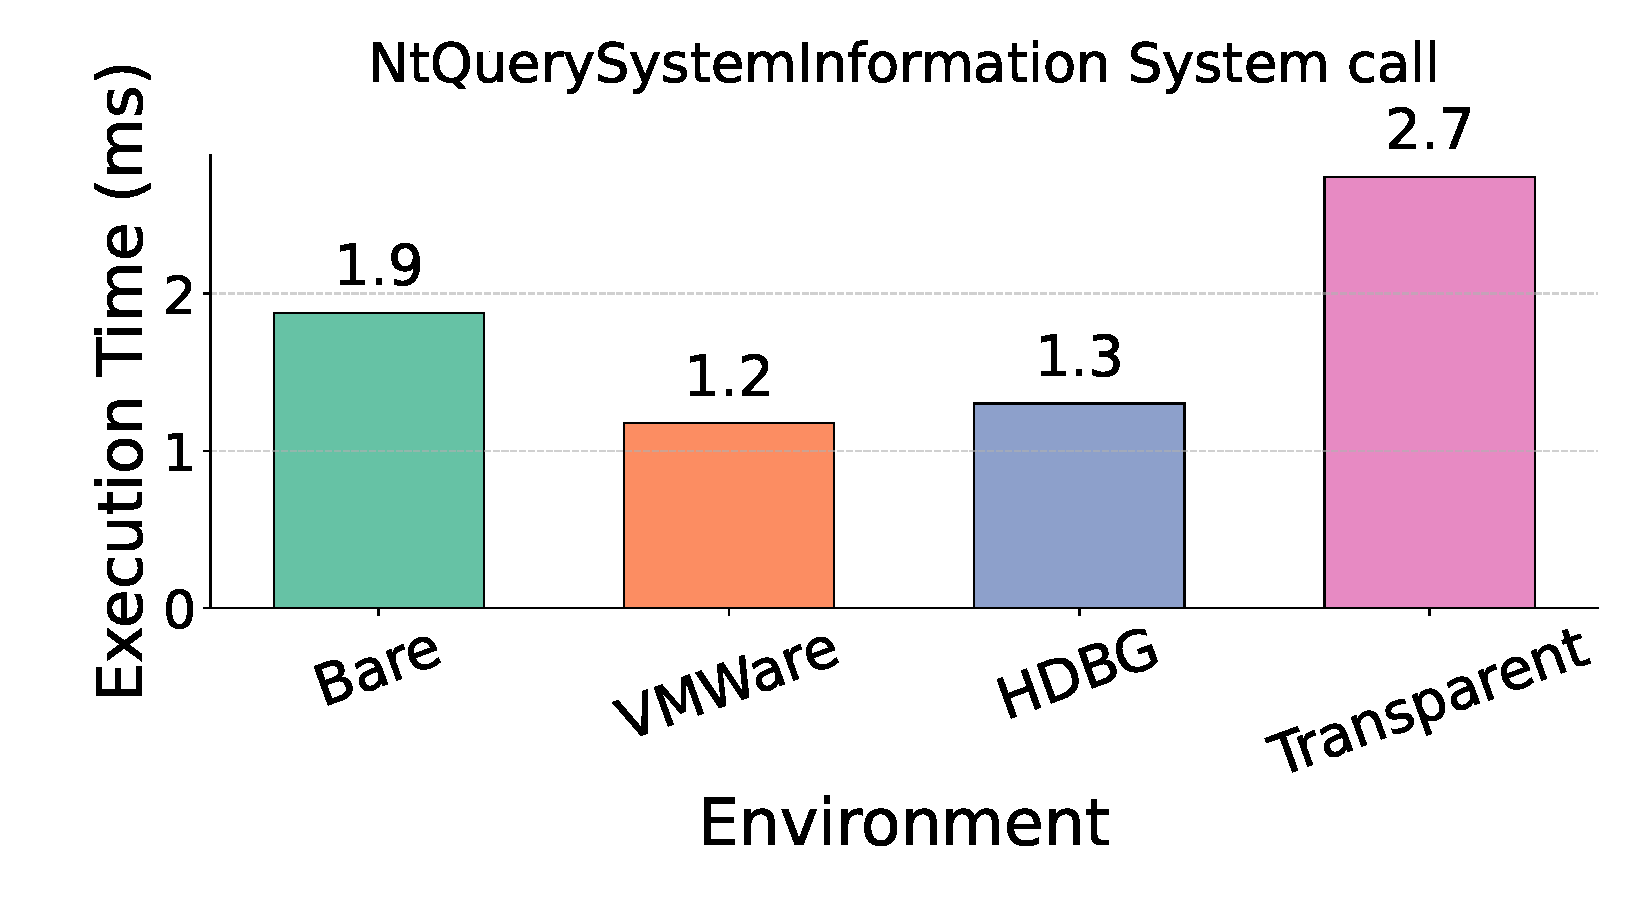
\includegraphics[width=\linewidth]{QSI execution}
        \sfigcap{}\label{fig:exec-time-c}
    \end{subfigure}
    \figcap{Execution time of Windows system calls in different environments. HyperDbg is shortened to \stress{HDBG}, and the data for the detection mitigation transparency mode is labeled as \stress{Transparent}.}\label{fig:execution_time}
\end{figure*}

The real performance impact can be seen in system call interception~\ref{fig:execution_time}. In graph~\ref{fig:exec-time-c} 
the measurements were taken for the NtSystemDebugControl system call. 
This is used by Microsoft debuggers, but can also be used to detect them, including HyperDbg. The transparency mode intercepts this call 
and changes its return value to an error code. A large increase in overhead can also be seen for the NtQueryKeyValue system call~\ref{fig:exec-time-a}, 
for a query of a registry key that would contain hypervisor specific data in its value, if it is read on a virtualized system.
Here the change in execution time is not as large, only 746\% versus the 1240\% increase for NtSystemDebugControl, but the average execution time is a lot longer, in general.

Interestingly, the execution of NtQuerySystemInformation, with a query for the SystemProcessInformation class, reveals less overhead that the other system calls, 
with only a 70\% increase. The lack of more noticeable overhead is because the mitigation for this specific query(\stress{SystemProcessInformation}) 
only requires reading and modifying a user-space memory buffer after the kernel has executed the SYSRET instruction. In contrast, mitigations for NtQueryKeyValue 
also require reading a user-space buffer before the kernel execution, to check the name of the registry key queried. 
The reason for the longer average execution time on the bare metal system is the increased active process count when the tests were performed, increasing the write times in the kernel.

From the intercepted system calls within the transparency mode, NtSystemDebugControl has the smallest code overhead. 
The handler only sets the trap flag for the callback function, in which only the return value in RAX is changed. 
This allows measuring just the overhead introduced by the 2 VM-exits plus the setting of the trap flag, which all the intercepted system call handlers perform. 
With a small error, the transparency overhead visible in graph~\ref{fig:exec-time-a}, is primarily this base overhead introduced by the EPT hook and trap flag VM-exit handlers. 
All system calls handled in the transparency mode will have this base time as the minimum overhead, with additional time delays introduced by memory reads, writes 
as well as any other logic executed in the handler functions.

The time overhead introduced by intercepting the system calls can be measured by malware or any other process in a similar way to how the VM-exit overhead is measured~\ref{HV_detection}. 
This is an issue that needs to be taken into consideration when the hypervisor detection methods are applied to malware analysis or any other process disassembly.

\subsection{Hypervisor Detection}\label{HV-detection-eval}
For the evaluation of the efficiency of the developed hypervisor transparency system, HyperDbg with the transparency mode enabled was deployed against tools that perform many of 
the common hypervisor and debugger detections tests. As a metric, the percentage of positive tests for each tool was measured and compared against running them on HyperDbg 
without the mitigations enabled. These tests were also run on a bare metal system for a base level and false positive measurement. 
The tools chosen for this evaluation were VMAware~\cite{vmaware}, Pafish~\cite{pafish}, and Al-khaser~\cite{al-khaser}, all of them perform numerous known hypervisor and debugger detection methods, 
most of which are also commonly used in malware. At the time of writing this paper, all 3 are still actively maintained and contain up-to-date detection methods.

Firstly, all of the tools were run on a bare metal machine to test for a base level and detect any false positives that might appear later on. 
Both VMAware and Pafish had 0 positive detections, but Al-khaser showed 1 false positive detection for the Local Descriptor Table(LDT) location test, 
so for the further tests in the virtualized environments, this test was disabled.

Running the testing suites on a VMWare guest system with HyperDbg deployed, but without the transparent mitigations enabled, yielded 16/111 positive detections or 14.41\%, 
Pafish tested 9/58(15.52\%) positive and running Al-khaser resulted in 48/327 positive tests or 14.67, Figure~\ref{fig:test_accuracy}.
It should be noted that many of the tests from all three tools are checking for presence of common consumer virtual machine providers like VMWare and VirtualBox signatures, 
so a lot of the tests performed use the same detection technique, just with different parameters, or searched strings, for these kinds of tests only the VMWare related ones could potentially get a positive score. 
The transparency mode was then enabled, and the same 3 hypervisor detection tools were run. VMAware positively detected only 10/111 (9.01\%) techniques, Pafish caught 6/58 (10.34\%) detection methods, and 
Al-khaser detected the hypervisor in 30 out of 327 attempts, which is 9.17\%, Figure~\ref{fig:test_accuracy}.
\begin{figure}[tbh]
    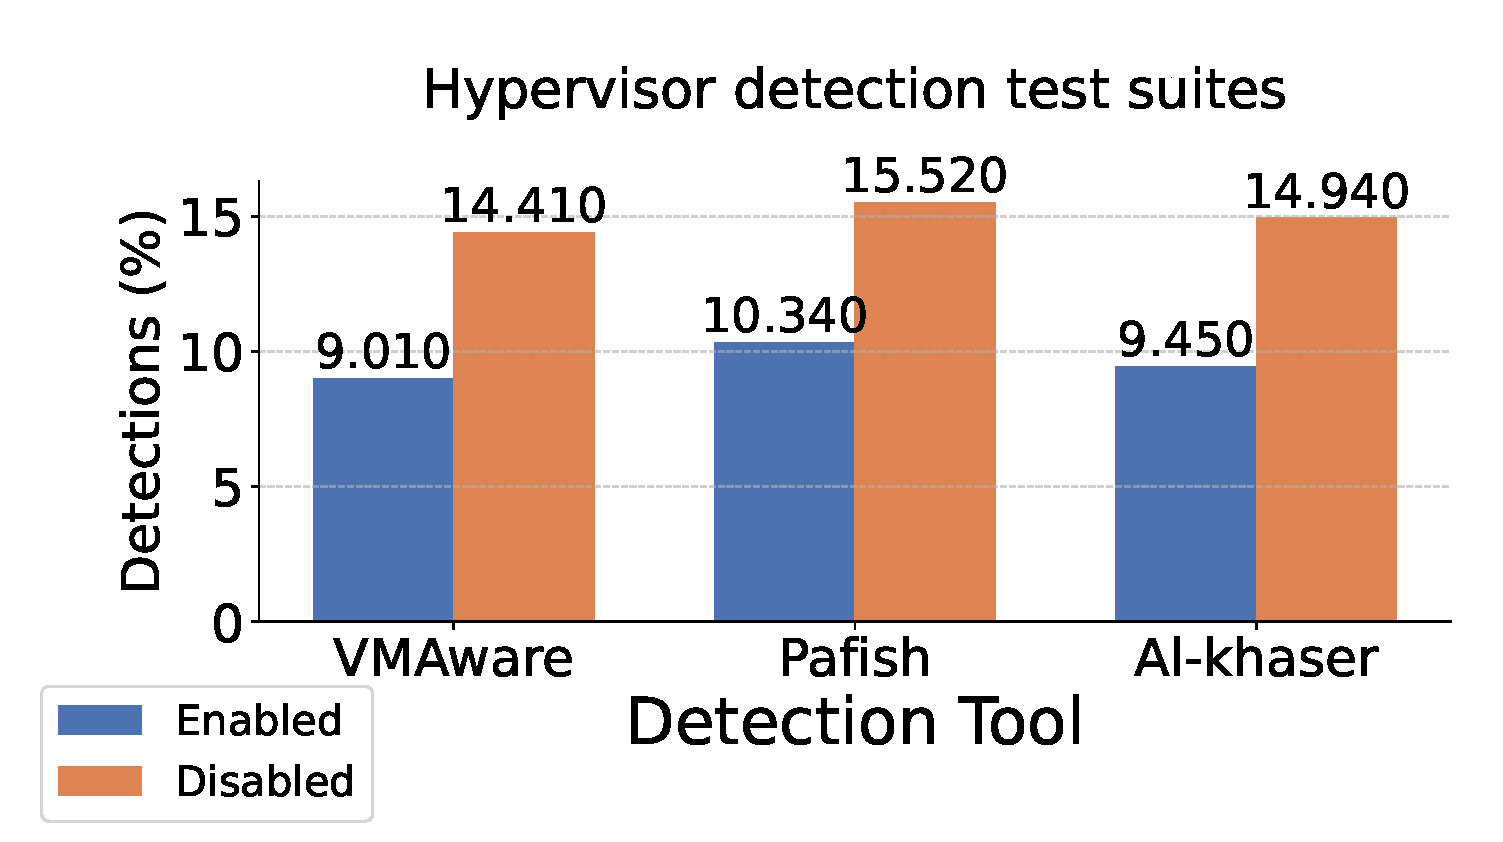
\includegraphics[width=\onecolgrid]{Accuracy tools} %RDTSC_execution
    \figcap{Percentage of positive detections from 3 hypervisor detection suites. \stress{"Enabled"} and \stress{"Disabled"} refer to the transparency mode of HyperDbg being enabled or not during the tests.}\label{fig:test_accuracy}
\end{figure}

Overall, the hypervisor detection mitigation system designed during this project yielded a 37.47\%, 33.38\% and 36.75\% improvement in transparency, 
with a 35.87\% overall average. These test suites primarily tested the system call approach to hypervisor detection and used many of the system calls that had handlers implemented as part of this paper, 
all of these test methods were successfully mitigated. But since this paper only tackled a small number of Windows system calls, there were still some detection vectors that had not been intercepted, 
as an example, the system firmware information available from reading a certain registry key\footnote{Information on firmware data available in the Windows registry. Microsoft. \url{https://learn.microsoft.com/en-us/windows-hardware/drivers/install/registry-trees-and-keys}} 
or from NtQuerySystemInformation with the SystemFirmwareTableInformation class. This structure was chosen not to be intercepted, and so, 
an attempt to read it from a virtualized system would still reveal hypervisor presence.

Evaluating the efficiency of the transparency features revealed the minimal instability in the implementation. The source of the system instability 
could not be definitively identified, but it caused only rare system crashes, and could not be measured.


\subsection{Comparison with ScyllaHide}\label{scyllahide-comparison}
HyperDbg is not just a hypervisor, it is also a kernel-space debugger~\cite{karvandi2022hyperdbg}. This means that during the design of 
the hypervisor transparency features, mitigating debugger detections was also taken into consideration. The approach of intercepting Windows system calls 
from the kernel-space allows HyperDbg to stay undetectable from any user-space process. ScyllaHide is a tool for debugger detection mitigation~\cite{scyllahide}, 
which stays in the user-space, and while it can mitigate most attempts at detecting a kernel-space debugger, ScyllaHide can only intercept API calls at the user-space level. 
This could allow detection attempts to bypass ScyllaHide by calling specific Windows system calls directly, avoiding the NT API interception. 

In the design proposed in this paper, the system call interception resides at the kernel level (level 0), with the mitigations performed at level -1, 
so even the direct system call invocation would be mitigated. To test this, a simple C++ program was created that called a specific Windows system call, 
NtSystemDebugControl. Firstly, using the NT API wrapper function with the same name and then directly, by emulating the API wrapper function.
\begin{listing}[!ht]

\begin{minted}[linenos,frame=single]{nasm}
    MOV R10, RCX
    MOV EAX, 0x01D0 ; System call number
    SYSCALL
    RET
\end{minted}
\caption{Windows system call wrapper function for NtSystemDebugControl from the NTDLL library.}
\label{lst:syscall-wrapper}
\end{listing}
When ScyllaHide was deployed and attached to the process of the created testing program, only the API call version could be intercepted and mitigated, 
while any tests calling directly to the kernel could bypass the transparent mitigations of ScyllaHide.
On the other hand, when HyperDbg's transparency mode is enabled and deployed on the system. Performing the same tests, both attempts can be intercepted and 
successfully mitigated.



%%% Local Variables:
%%% mode: latex
%%% TeX-master: "../thesis"
%%% End:

\section{Discussion}\label{s:discussion}

%%A “limitations” section, as the name implies, describes scenarios where the
%%proposed solution may not work well. Although a “discussion” section could also
%highlight limitations of the proposed work, it focuses on analyzing the
%implications of the proposed work for current and future research.

\subsection{Design Limitations}
The implemented detection mitigations are system wide; this provides the best level of transparency, even in the case of an attempt 
to perform these detection checks on a different process. The downside of this approach is that it will also interfere with normal, 
genuine processes that expect certain data or values to be present, like the VM support programs many commercial hypervisor vendors use, 
which might store crucial data in locations blocked by these transparency features. As well as Windows processes that expect no kernel modifications. 
As an addition to the transparency mode in HyperDbg, a two stage transparency, with a semi-transparent mode added, would improve the usability and reliability of the hypervisor. 
In this system, a select number of processes are allowed to bypass all transparent mitigations as well as not intercepting the MSR accesses that could cause instability. 
As a trade-off, this semi-transparent mode would allow malware to more easily run successful hypervisor detections and avoid full analysis, by emulating the appearance of one 
of these genuine, whitelisted processes.

The system call interception of the mitigation design is based on filtering the system calls based on their system call numbers~\ref{tab:syscalls} and thus the mitigations 
only work if deployed on a guest system that runs the correct Windows version, as Microsoft is known to change the system call numbers between versions 
frequently~\cite{j00ruSyscalls}. In an implementation of the system call interception, an ability to obtain these system call numbers is needed for correct operation.
Within HyperDbg, obtaining the current Windows version of the guest is possible, and a feature to get the system calls of the guest OS version was also implemented, but not as a part of this thesis.

\subsection{Not Full Transparency}
This thesis only covered 3 general hypervisor detection vectors, there are numerous other ways any user-space process could detect the virtualized environment, 
and a fully transparent and reliable hypervisor is nearly impossible to create. Deploying HyperDbg with the transparency features from this thesis does not guarantee any true 
transparency, and it can remain stealthy if the malware or any other binary analyzed only uses the detection methods discussed in this thesis.

The implemented transparency features also leave detectable traces of their own, and a process developed with HyperDbg in mind could find these 
traces and still detect the virtualized environment of HyperDbg's hypervisor. The remaining artifacts include inconsistent return values, memory buffers 
that are not the correct size, or inconsistencies between the same data obtained from different sources, like a system call which does not get intercepted by HyperDbg.

While guaranteeing 100\% transparency is not feasible, the design created during this thesis significantly raises the bar and makes it more difficult for malware to defeat these anti-anti-hypervisor techniques.



%%% Local Variables:
%%% mode: latex
%%% TeX-master: "../thesis"
%%% End:

\section{Related Work}\label{s:related}

It is quite unlikely that you were the first to address this problem. Please use
this section, hence, to discuss what prior work had done and how your solution
is different from or better than prior work. You may place this section
immediately after the “Background” section, if necessary.

\textcolor{lightgray}{\lipsum[26-29]}

Srinivasan Keshav's old---but still relevant---article on how to read a paper
might be quite useful for also reviewing prior work~\cite{Keshav-SIGCOMMCCR2007}.


%%% Local Variables:
%%% mode: latex
%%% TeX-master: "../thesis"
%%% End:

\clearpage
\section{Conclusion}\label{s:conclusion}

In this thesis, we have discussed the many ways of detecting the presence of hypervisors on the running system from a user-space process, 
the use and prevalence of these detection methods in malware, as well as designed mitigations for these detections that can be added to any hypervisor to make it more transparent and stealthy. 
By intercepting requests for data that are known to contain information revealing hypervisor presence, like certain CPU instructions or system calls of the operating system, 
and modifying the data the calling user-space process receives, it is possible to hide the presence of any hypervisors on the system. 
These hypervisor transparency features were then implemented into HyperDbg, a hypervisor based debugging tool, and the effectiveness of the mitigations was 
tested against the hypervisor detection attempts using tools that compile these detection methods and perform tests with all of them. By evaluating the designed mitigations, 
it was shown that enabling the transparency mode in HyperDbg not only improved the stealthiness of HyperDbg, the underlying hypervisor on which HyperDbg was nested on top also 
became harder to detect.

The hypervisor transparency features developed as part of this thesis are only a small portion of the numerous ways the presence of hypervisors can be detected. 
As with most cybersecurity development, full security and protection cannot be guaranteed. The development was done in a highly modular and expandable fashion, 
to allow future additions and improvements to hypervisor transparency in HyperDbg, as more mitigation methods are developed and new ways to detect hypervisors are discovered. 



%%% Local Variables:
%%% mode: latex
%%% TeX-master: "../thesis"
%%% End:


\bibliographystyle{ACM-Reference-Format}
\bibliography{references}

\clearpage
\appendix
\section*{Artifacts}\label{s:artifact-appendix}

Based on the standard Artifact Appendix template used by the USENIX Security
Symposium. Please follow the self-contained instructions below and assume
(i)~you are compiling the final version of the Artifact Appendix (no need to
cater to reviewers, but to general users of your artifact) and (ii)~you are
documenting everything in scope for all the artifact evaluation badges
(\emph{Artifacts Available}, \emph{Artifacts Functional}, \emph{Results
Reproduced}). More information at~\cite{secartifacts}.

%%%%%%%%%%%%%%%%%%%%%%%%%%%%%%%%%%%%%%%%%%%%%%%%%%%%
% Artifact Appendix Template for Usenix Security'24 AE
%%%%%%%%%%%%%%%%%%%%%%%%%%%%%%%%%%%%%%%%%%%%%%%%%%%%

\section{Artifact Appendix}

%%%%%%%%%%%%%%%%%%%%%%%%%%%%%%%%%%%%%%%%%%%%%%%%%%%%%%%%%%%%%%%%%%%%%
\subsection{Abstract}
{\em During this thesis, multiple hypervisor detection mitigation approaches were discussed and designed. These mitigation methods were then implemented into HyperDbg, 
developing the transparency mode of HyperDbg. The transparency features attempt to hide the HyperDbg hypervisor and any other virtualized environment HyperDbg has been nested on top of, 
by intercepting and modifying the data a calling user process will receive and are deployed from HyperDbg during runtime without requiring system reboot.}

%%%%%%%%%%%%%%%%%%%%%%%%%%%%%%%%%%%%%%%%%%%%%%%%%%%%%%%%%%%%%%%%%%%%%
\subsection{Description \& Requirements}

\textit{Both the development and evaluation of the hypervisor detection technique mitigation methods were carried out
on a Microsoft Windows 11 24H2 bare metal system as the host system, with a 10th generation Intel Core\textsuperscript{TM} CPU which supports VT-x hardware virtualization feature.
The virtualized guest system was run on this host using a VMWare Workstation 16 hypervisor with nested virtualization support enabled.
This guest system was used to run HyperDbg's hypervisor and perform all evaluation and testing. The development of the transparency features in HyperDbg was based on its 0.13.0 release version. }

\subsubsection{Security, privacy, and ethical concerns}
\textit{The containerized nature of virtual machines adds a layer of security to a bare metal system that is used as the host for malware analysis.
During this project, no actual malware samples were tested, only non-malicious parts of them, so full host system safety cannot be guaranteed from this thesis.
To be able to run HyperDbg's hypervisor, Windows Driver Signature Enforcement security feature as well as VBS(Virtualization Based Security) must be disabled on the guest system.
This allows the loading of unsigned drivers, which HyperDbg's hypervisor driver is, but it also allows any other process to load their unsafe drivers, 
exposing the system to a much lower level and harder to detect malware attacks. HyperDbg itself, including the features implemented as part of this thesis, are open source and available under the GNU GPL v3.0 copyleft license.}

\subsubsection{How to access}
\textit{Access to the developed transparency features is freely available on GitHub, as part of the HyperDbg project~\cite{hyperdbg}. 
The individual commits to intermediate feature implementations are available at: CPUID transparency \href{https://github.com/HyperDbg/HyperDbg/commit/56c2d400fddca22f314c1e5d16cadce6950eb262}{Link}, 
MSR transparency \href{https://github.com/HyperDbg/HyperDbg/commit/2cc3da3daebd793fd56d5c370ef6da398efa6d29}{Link}, Windows system call
transparency \href{https://github.com/HyperDbg/HyperDbg/commit/d0610661baf944259c33e921d3fc265e6a217ad8}{Link}
}


\subsubsection{Hardware dependencies}
\textit{To be able to evaluate the hypervisor transparency features implemented as part of this thesis.
The system running the hypervisor driver must have an Intel x64 CPU which supports VT-x and EPT technologies. As of writing this thesis, AMD CPUs are not supported.
Both the host and guest systems should also have at least a serial port each that are connected together, this can be a physical connection or a virtual one in case of nested virtualization usage.}

\subsubsection{Software dependencies}
\textit{Both the host and guest systems must be running the 64 bit version of Microsoft Windows operating system,
a certain release version is not specified, but testing was done, and correct operations can only be guaranteed, on Windows 11, with most of the functionality also remaining in Windows 10.
HyperDbg can be obtained as a compiled software, so no compilation is needed. To be able to load the hypervisor driver of HyperDbg,
Driver Signature Enforcement feature needs to be disabled, one of the methods, and the one that was used during the evaluation section, involves the use of a third party tool WinDbg \href{https://github.com/HyperDbg/HyperDbg/commit/2cc3da3daebd793fd56d5c370ef6da398efa6d29}{Link}, but this is not required.}

\subsubsection{Benchmarks}
\textit{None}

%%%%%%%%%%%%%%%%%%%%%%%%%%%%%%%%%%%%%%%%%%%%%%%%%%%%%%%%%%%%%%%%%%%%%
\subsection{Set-up}

\textit{For this example evaluation, the nested virtualization approach is chosen, in this case the guest system on which the evaluation will be performed,
is a VMWare Workstation 16 virtual machine running Microsoft Windows 11 24H2. This is assumed to already be set up and in a working state. The precompiled HyperDbg package was used.}

\subsubsection{Installation}
\textit{To deploy the transparency features, only the guest VMWare system and HyperDbg is needed. The downloaded compiled HyperDbg package directory needs to be present on both the guest and host systems. 
Once HyperDbg has been deployed in kernel debug mode, following its installation guide available at: \href{https://docs.hyperdbg.org/getting-started/build-and-install}{Link}, the transparency mode, 
which contains the features developed, can be enabled by entering the "!hide" command in the CLI of the host system, and once the confirmation output is displayed, the hypervisor transparency has been enabled 
and the control can be returned to the guest with the "g" command. Now any user-space process attempting to call the CPUID instruction or querying one of the intercepted system calls 
will receive the mitigated output.}

\subsubsection{Basic Test}
\textit{The functionality of the hypervisor detection mitigation features can be tested by creating and running a simple program that queries the CPUID instruction with the EAX register set to 0x01
 and then reading the 31st bit of the returned value in RAX. This is the "hypervisor present" bit and in a normal virtual environment this bit would be set, but the transparency features unsets it, 
 to appear as if this is a bare metal system.}

%%%%%%%%%%%%%%%%%%%%%%%%%%%%%%%%%%%%%%%%%%%%%%%%%%%%%%%%%%%%%%%%%%%%%
\subsection{Evaluation workflow}

\subsubsection{Major Claims}
The major claims made during this thesis.\\

\begin{compactdesc}

    \item[(C1):] \textit{A virtual system with the hypervisor detection mitigations enabled is more transparent and the hypervisor is harder to detect from the user-space. 
    This is proven in section~\ref{HV-detection-eval} by evaluating the designed mitigation system against third party tools that execute commonly used hypervisor detection techniques. 
    The improvement can be seen in Figure~\ref{fig:test_accuracy}}

    \item[(C2):] \textit{The designed system for Windows system call interception is more resilient than other approaches used by similar implementations like ScyllaHide. Section~\ref{scyllahide-comparison}
    proves that intercepting system calls at the kernel level improves the resiliency of the mitigations. 
    A process making a system call directly to the kernel bypasses the interception attempts in the design of ScyllaHide, but the system designed in this thesis, in Section~\ref{syscall_interception} can still intercept it}

\end{compactdesc}

\subsubsection{Experiments}
\textit{The experiments performed for the evaluation of the designed transparency features. Corresponding to the major claims made in the previous section.
For all of the experiments below, HyperDbg is deployed in kernel debug mode and active during them, with the transparency mode disabled, unless stated otherwise.}

% use paralist for more compact list format: for more details check here:
% https://texfaq.org/FAQ-complist
\begin{compactdesc}

    \item[(E1):] \textit{Evasion efficiency:
    The experiment consisted of running one of the 3 chosen hypervisor detection tool suites on the virtualized system running HyperDbg with the transparency mode disabled as well as enabled}

    \begin{asparadesc}
        \item[How to:]  \textit{Once HyperDbg has been successfully deployed on the guest system, the detection suite is run on the guest. The result given by the tools vary, but all of them will contain 
        a number of positive detections over the total count of detection methods performed. This score can then be logged and the transparency mode can be enabled. Once it is enabled, the same tool can be run again 
        and the, now much smaller, score can also be logged and compared to the previous one.}

        \item[Results:] \textit{The results should show a decrease in positive detections when they were performed with the transparency mode enabled. For a more clear comparison, the two percentage values can also
        be plotted, as it can be seen in Figure~\ref{fig:test_accuracy}.}
    \end{asparadesc}

    \item[(E2):] \textit{Syscall interception:
    For this experiment a custom program needs to be created that calls a specific Windows system call in two different ways and displays the return value.}

    \begin{asparadesc}
        \item[How to:]  \textit{This experiment requries the creation of a small program that calls the NtSystemDebugControl systemcall in two different ways, once by calling the NT API function of the same name
        and then calling directly to the kernel by executing the SYSCALL assembly instruction like seen in Listing~\ref{lst:syscall-wrapper}.}
        
        \item[Preparation:]  \textit{To compare the design of the mitigations, ScyllaHide needs to be obtained from its source and made available to the guest system. The same goes for any debugging tool that can
        can be used to attach itself to the process of the testing program. The aforementioned program also needs to be created and available.} 
        
        \item[Execution:]  \textit{Firstly, ScyllaHide can be deployed, by attaching its library to the process of the testing program, using the provided CLI. Then the debugger should also be attached to the same 
        process. The system call test can then be executed, and after the returned values are shown, it should be noticeable  that ScyllaHide can only intercept the API based call and not the direct kernel system call.
        After this the same process can be repeated without attaching ScyllaHide, but enabling the transparency mode in HyperDbg.}
        
        \item[Results:] \textit{The results should show ScyllaHide only intercepting and mitigating the first approach of the system call calling, while HyperDbg's transparency mode is able to intercept and mitigate both
        calling approaches.}
    \end{asparadesc}

    \item[(E3):] \textit{[Optional Name] [1 human-hour + 3 compute-hour]: ...}

\end{compactdesc}

%%%%%%%%%%%%%%%%%%%%%%%%%%%%%%%%%%%%%%%%%%%%%%%%%%%%%%%%%%%%%%%%%%%%%
\subsection{Notes on Reusability}
\label{sec:reuse}

\textit{The hypervisor detection mitigation features, as implemented into HyperDbg, can allow more reliable dynamic malware analysis when using HyperDbg.}

\textit{These features, developed as part of this thesis, are only a small portion
of the numerous ways that the presence of hypervisors can be detected. As with most cybersecurity development, 
full security and protection cannot be guaranteed. The development was done in a highly modular and expandable fashion, 
to allow future additions and improvements to hypervisor transparency in HyperDbg, as more mitigation methods are developed and new ways to detect hypervisors are discovered.}

%%%%%%%%%%%%%%%%%%%%%%%%%%%%%%%%%%%%%%%%%%%%%%%%%%%%%%%%%%%%%%%%%%%%%

\subsection{Version}
%%%%%%%%%%%%%%%%%%%%
% Obligatory.
% Do not change/remove.
%%%%%%%%%%%%%%%%%%%%
Based on the LaTeX template for Artifact Evaluation V20231005. Submission,
reviewing and badging methodology followed for the evaluation of this artifact
can be found at \url{https://secartifacts.github.io/usenixsec2024/}.

%%% Local Variables:
%%% mode: latex
%%% TeX-master: "../thesis"
%%% End:


\end{document}


%%% Local Variables:
%%% mode: latex
%%% TeX-master: t
%%% End:
